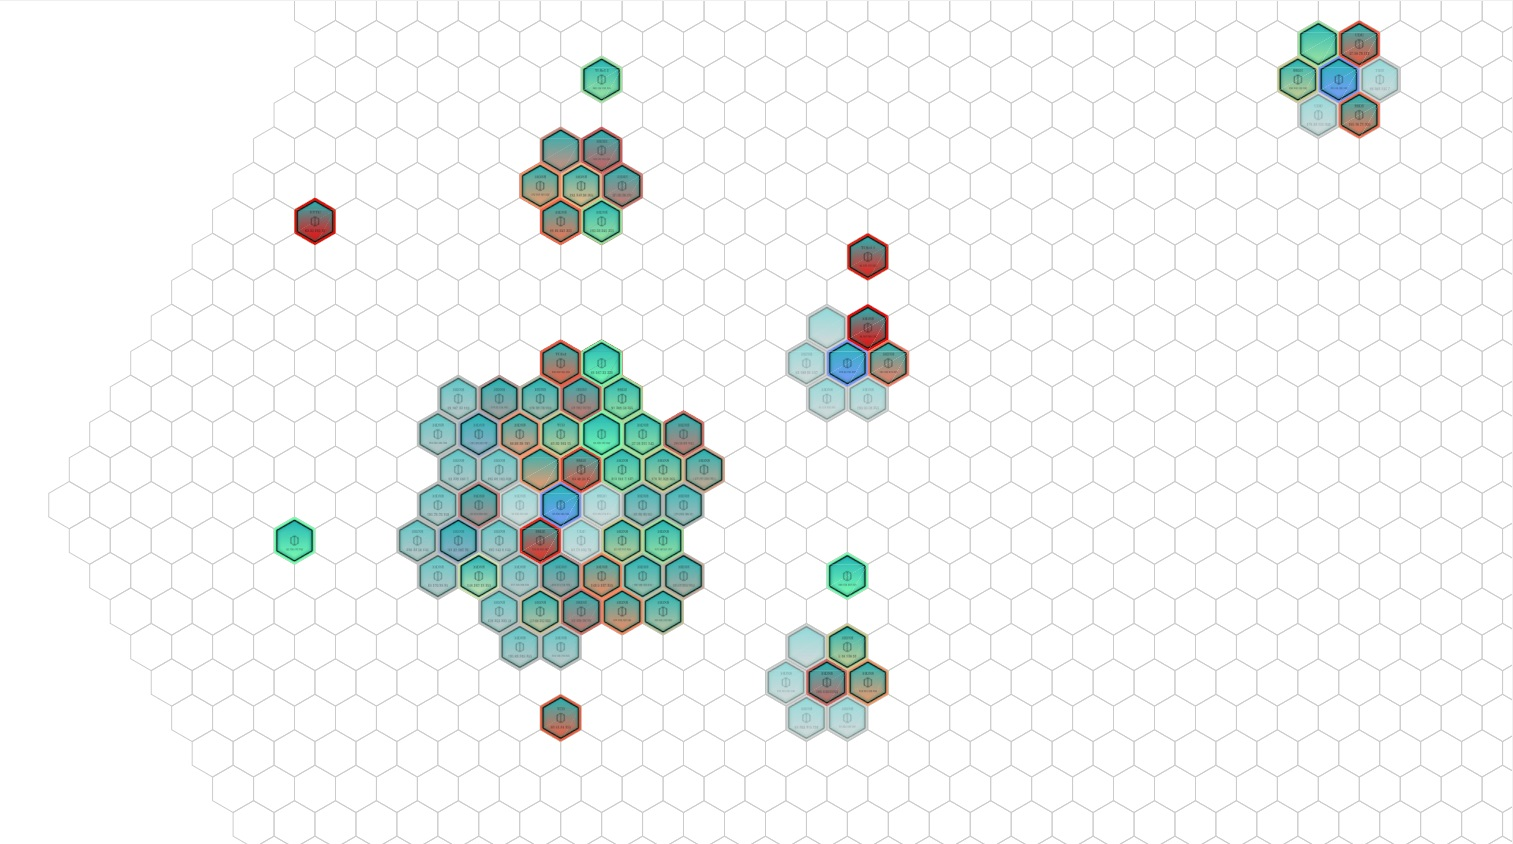
\includegraphics[width=\linewidth]{materials/groups.jpg}
This visualization also makes use of the hexagonal grid. In the attempt to give
a best possible insight it uses two visual factors: size and proximity.

As the traffic in the network rises, the nodes representing machines are put on
the map. All the machines sending packets to one specific device are grouped
together. As more machines communicate with a specific address, more nodes
appear around the hexagon representing their destination. Node placement is
automatic. The procedure ensures that there is enough space around a centre
and that no two nodes overlap.

The colour of the communicating nodes represents how much data they send. More
heavily used destinations will thus have more orange and red nodes around them,
and destinations used by a lot of machines will have a greater number of nodes
around them. Therefore nodes receiving more traffic are easier to spot.

This visualization helps detect the machines that perform a server role in the
network. It also allows a user to quickly identify what type of service the device
is providing. Each node specifies the most commonly used protocol, thus
revealing the possible role of the machine in the network.

